% GENERATED FILE -- do not edit.
% Produced by paper/make_agentverify.py from paper/main_short.tex.
% Anonymous IEEE conference version for a double-blind workshop submission.
% Edit main_short.tex and regenerate; check_consistency.py enforces that this
% file matches its source.
\documentclass[conference]{IEEEtran}
\IEEEoverridecommandlockouts
\usepackage{amsmath,amssymb,booktabs,enumitem,tabularx,array,graphicx,xcolor}
\usepackage{url}
\usepackage[numbers,sort&compress]{natbib}
\usepackage{stfloats}
\usepackage[hidelinks]{hyperref}
\newcommand{\gzero}{g{=}0}\newcommand{\DeltaAUROC}{\Delta\mathrm{AUROC}}

\title{Auditing the Winner: Evaluate Failure Detectors on the\\ Population the Selector Actually Commits}
\author{\IEEEauthorblockN{Anonymous submission}\IEEEauthorblockA{Paper under double-blind review}}

\begin{document}\maketitle


\begin{abstract}
When an agent commits the best of $n$ attempts under a critic, the committed trajectory is where the critic's confidence and its errors coincide. A common proposal is to audit it with a disjoint panel of critics and escalate on disagreement. Audit signals are usually evaluated over candidate pools, but a deployed auditor runs \emph{after} selection, so we evaluate this one on the population a selector actually commits, against the selector's own score, with executed gold. We pre-registered and ran it on SWE-bench Verified (41 instances, 9 repositories) and SWE-bench Multilingual (114 instances, 37 repositories): best-of-4 selection by a reward model, a checkpoint-disjoint panel, and the official test harness. Silent failures --- committed, agent-declared-complete trajectories that fail hidden tests --- were 35\% and 45\% of the population. The registered endpoint is the out-of-fold gain in AUROC from adding panel disagreement to the selector's own score. On it, disagreement adds nothing detectable: pooled over 47 failures and 46 repositories, the three estimators that use every row give $-0.03$, $-0.01$ and $+0.01$, every interval includes zero, and the loosest pooled upper bound is $+0.12$. This held across 4k--16k contexts, pruned windows, eight reward models from 1B to 32B, two re-selection regimes and a panel of LLM judges, and the pilot's positives did not replicate on 37 fresh repositories (Fig.~\ref{fig:replication}): $u_{\max}$ fell from 0.686 to 0.541 and the 1B critic from 0.712 to 0.485. Individual judges are the exception --- \texttt{gpt-6-sol} ranks failures at 0.776 [0.68, 0.87] --- but their disagreement is not. Why the population matters: on Verified the selector's own score ranks failures at 0.81 among candidates it passed over and 0.61 among those it committed, so pool performance does not answer the deployment question. We did not detect increased failure under selection, and we report a bound rather than an absence.
\end{abstract}

\section{Introduction}
Best-of-$n$ selection under a learned critic is a default in agent scaffolds: generate several trajectories, score each with a reward model, commit the argmax. Three claims about this are easy to conflate, and this paper keeps them apart. The \emph{theory} is that argmax selection on a noisy score induces the optimizer's curse~\citep{smith2006optimizer}: the top-scored candidate is disproportionately the one whose flaws the critic cannot see, so the score carries less information about the committed candidate than about the pool. What we \emph{observe} is one instance of that theory measured directly: on Verified the selecting critic ranks failures at 0.81 among candidates it passed over and 0.61 among those it committed, on the same instances. What we do \emph{not} show is that selection raised the failure rate of the committed candidate --- with the selector we used, it did not (\S\ref{sec:control}). A committed trajectory that fails while carrying a high score is a \emph{silent failure}; they are a third to a half of what this agent committed, whether or not selection put them there.

The obvious safeguard is a second opinion. If a panel of critics disjoint from the selector disagrees sharply about a committed trajectory, that disagreement might carry information the selector has exhausted. That correlated critics share blind spots is not our idea: the correlated-judge literature predicts it~\citep{goel2025great,kim2025correlated,kohli2026nine,hossain2026agreement,afrin2026ensembles}, and best-of-$n$ reward hacking is well characterised~\citep{gao2023scaling,khalaf2025inference,yu2026caution}. What had not been done is the measurement: put a disjoint panel on the population a critic actually committed, with executed gold, structural baselines and pre-registered bars, and ask what it adds over the selector. Our contributions:
\begin{itemize}[leftmargin=1.2em,itemsep=0pt]
\item \textbf{A selection-conditional evaluation protocol for audit signals} --- selected population, selector baseline, executed gold, pre-registered bars --- with its first two-benchmark instantiation on SWE-agent trajectories. Candidate-pool discrimination does not measure residual auditing value on the selected population~\citep{emadi2026scaling,trilemma2026}.
\item \textbf{A replicated lack of detectable gain with an estimator-robust bound}: disagreement's incremental value is indistinguishable from zero under four estimators, loosest pooled upper bound $+0.12$ over 47 positives and 46 repositories.
\item \textbf{Diagnostics}: test--retest stability of long-window reward-model scores, the repository-clustering ceiling on effective $n$, and seven instrument failures that each would have produced a false positive (\S\ref{sec:instrument}).
\end{itemize}
``Critic'' means an off-the-shelf reward model or LLM judge used without task-specific training. Trained trajectory verifiers~\citep{shum2025swerm,rahman2026scout,wang2026failfast} are a different class.

\paragraph{Setup}
The unit is one committed trajectory. Gold $g\in\{0,1\}$ is trajectory-level success under the official \texttt{swebench} 5.x harness; the positive class is failure ($\gzero$). The selecting critic $c_{\mathrm{sel}}$ scores each of $n{=}4$ full candidates and commits the argmax; the audit panel $\{c_1,\ldots,c_m\}$ satisfies $c_{\mathrm{sel}}\notin\{c_i\}$ at checkpoint level, and $u$ is the sample standard deviation of their rank-normalised scores, with rank norms fit on training repositories only. The population is committed trajectories whose agent exited with a submission and a non-empty patch. M1 $=\mathrm{AUROC}(u)$, M2 $=\mathrm{AUROC}(-c)$, M3 $=$ M1 $-$ M2 with a repository-clustered bootstrap. Population, positive class, metrics, predictions and a stopping rule were committed to a version-controlled pre-registration before any gold existed; each later analysis was added as a dated amendment before its data existed.

\section{Silent failures are common; increased failure under selection was not detected}\label{sec:control}
\begin{figure*}[t]\centering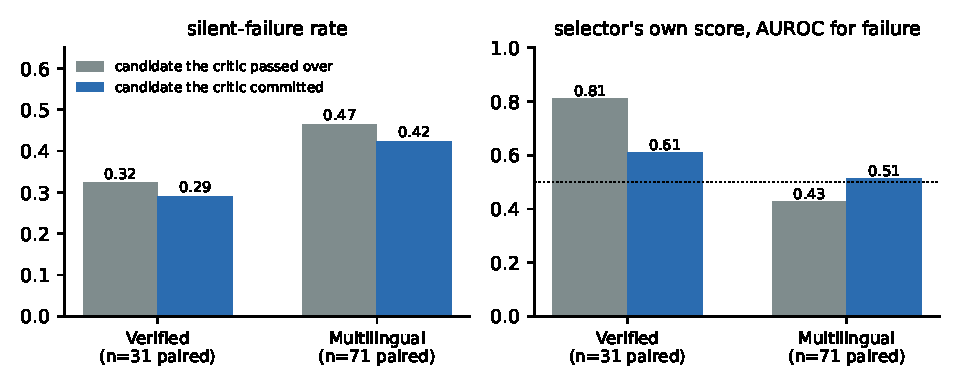
\includegraphics[width=0.92\linewidth]{figures/fig_control.pdf}
\caption{\textbf{Picking did not make things worse --- but it did use up the picker's own judgment.} One candidate the critic passed over, graded per instance, paired with the one it committed.}\label{fig:control}\end{figure*}
Of 164 Verified candidates, 138 exited having submitted; selection by \texttt{Skywork-Reward-V2-Qwen3-4B} committed 34 usable trajectories, of which the harness resolved 22 and failed 12: \textbf{35.3\% [21.5, 52.1] silent failures}. On Multilingual the same pipeline gave 77 usable rows and 35 failures (45.5\%). Selection was real (the chosen index spread across all four slots) and $\mathrm{corr}(c,u)=0.11$. One incidental measurement bounds what \emph{any} auditor on this benchmark can be checked against: the median analysed instance is guarded by exactly one \texttt{FAIL\_TO\_PASS} test, and 84 of 111 analysed rows are guarded by exactly one (22 of 34 on Verified, 62 of 77 on Multilingual). ``Resolved'' is usually a single test's verdict, so the label our AUROCs are computed against is thinner than the word suggests.

Whether selection \emph{concentrated} failure is a separate question a committed-only sample cannot answer. Amendment 4f graded one unselected candidate per instance on both benchmarks (31 and 71 paired rows). Figure~\ref{fig:control} shows both arms. \textbf{We did not detect increased failure under selection}: $-3$ points on Verified [$-21$, $0$] and $-4$ on Multilingual [$-11$, $+3$]. \textbf{F-P1}, that selection concentrates failure, \emph{failed on both}; the Multilingual interval still admits three points more concentration, so this is a failure to detect rather than a demonstrated absence, and we claim a failure \emph{rate}, not concentration. \textbf{F-P3} registered no prediction and required only that disagreement on the random arm be reported: it is 0.367 on Verified and 0.51 on Multilingual, so the range-restriction reading --- disagreement working on an unselected pool while failing on the committed one --- is not available either. The control does measure the selection-conditional gap: on Verified the selector ranks failures among candidates it did not pick at 0.81 [0.74, 1.00] and among those it committed at 0.61 on the same instances. On Multilingual the critic has no signal in either arm (0.43, 0.51), so there was nothing to remove.

\paragraph{Disagreement does not detect them}
The primary analysis --- four chat-preference reward models auditing a 4{,}096-token prefix --- gave $\mathrm{AUROC}(u)=0.508$ against the selector's own 0.621. Every amendment was declared before its data existed and asked whether some limitation of the primary was hiding a signal: the final diff plus the last 3k tokens, the patch in view, a true 16k context, re-selection by the proposal's named 8B critic and by a code-trained model, \texttt{AceCodeRM-7B} and its 32B sibling, and a confirmatory panel of three \texttt{gpt-5}-family judges. Panel $u$ never left 0.439--0.686 (Fig.~\ref{fig:ladder}); the two panel values quoted here, 0.494 with the patch in view and 0.439 at 16k, are the registered four-member panel, not the six models scored individually. Individual judges did better: \texttt{gpt-5} reached 0.720 and \texttt{gpt-5-mini} 0.752, while their disagreement was 0.528. \texttt{gpt-5-mini} is also the agent, so its 0.752 is a self-evaluation; \texttt{gpt-5} is not, and clears the same bar at 0.720. That clearance triggers \textbf{A4c-P1}'s registered reading, under which the claim would narrow to \emph{reward-model} critics; we decline the narrowing, because the judge saw the diff and the reward models did not, and we label declining it post hoc. \emph{Every registered prediction that panel disagreement carries signal beyond the selector failed.} One registered bar was cleared and we disclose it: the primary hypothesis was registered as the bare inequality $\mathrm{AUROC}(u) > 0.5$, and $u$ is 0.508 and 0.565, so it passes as written. We do not treat it as a detector --- the bar carries no minimum effect size, both intervals include chance, and the paired comparisons are $-0.114$ and $+0.005$. Registering a threshold with no margin was our design error; overruling it is post hoc and labelled so. Two registered own-score predictions also fail: \textbf{P2} (Goodhart) required $\mathrm{AUROC}(-c)\le 0.5$ and fails at 0.621, and \textbf{A2-P1} required AceCodeRM-7B above 0.60 and fails at 0.405. One prediction, on the code-trained critic's prefix-versus-full-length correlation, is undecidable: that model fell back to 4k on 31 of 34 rows.
Figure~\ref{fig:ladder} plots all thirteen. Panel disagreement spans 0.439 to 0.686 across every variation of input length, critic size, critic identity, training signal, critic class and selection regime, against a selecting critic at 0.621 and a structural baseline at 0.665. The paired gain M3 is negative in nine of thirteen rows and no interval excludes zero; the widest upper bound anywhere in the sweep is $+0.63$, on the code-trained critic's 16k re-selection over eleven positives. Figure~\ref{fig:ladder} plots every row; the thirteen configurations are enumerated above.

One configuration crossed its bar. Amendment 3 pruned tool outputs and scored overlapping 3{,}500-token windows, taking the panel's maximum disagreement: $\mathrm{AUROC}(u_{\max})=0.686$ against a pre-registered bar of 0.665, with a free permutation $p=0.04$ that rises to $p=0.21$ within repository and a leave-one-instance-out range of 0.657--0.731 that straddles the bar.

\begin{figure*}[t]\centering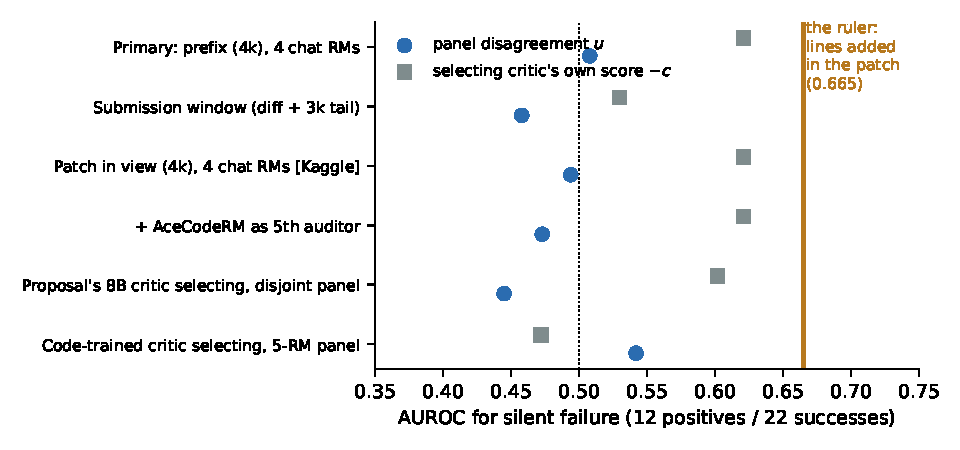
\includegraphics[width=\linewidth]{figures/fig_ladder.pdf}
\caption{\textbf{Every way we tried to make disagreement work, on the pilot.} Each row is one configuration; 0.5 is a coin flip. Circles are panel disagreement, squares the selecting critic's own score. The gold line is lines added to the patch: a baseline that needs no model at all. Exactly one circle crosses it: pruned-window $u_{\max}=0.686$, which failed to replicate. Exactly one square does: the 8B critic's own score at a true 16k, 0.736.}\label{fig:ladder}\end{figure*}

\paragraph{A ruler beats the critics} Two integers read off the diff and the transcript, with no model involved, rank silent failures better than every reward model at 4k and every single-window disagreement statistic at any length: lines added, 0.665, and agent step count, 0.657 (Fig.~\ref{fig:ladder}). We propose lines-added as the bar any audit statistic must clear before it earns a confirmatory run. It is a screening baseline and not a deployable guardrail, since an agent optimising against it would simply write shorter patches; \S\ref{sec:replication} shows it does not survive the replication either, which is the point.

\section{Replication on 37 repositories}\label{sec:replication}
\begin{figure*}[t]\centering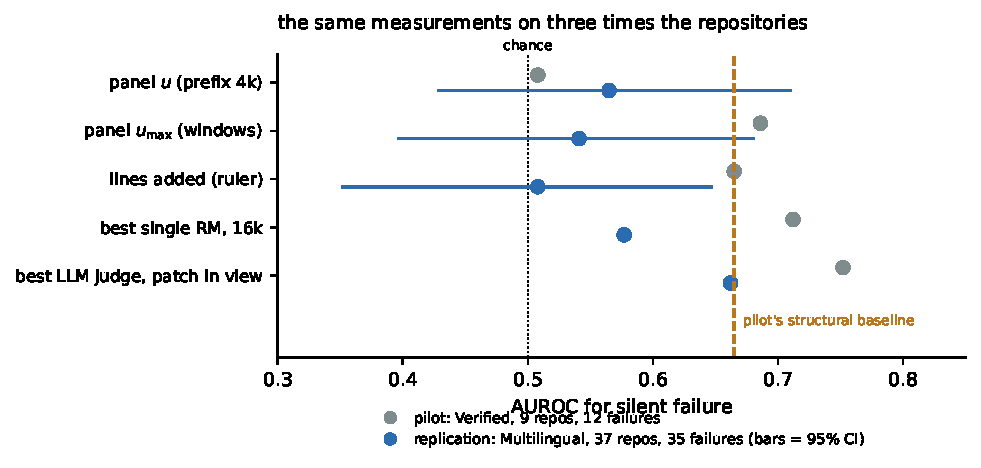
\includegraphics[width=0.92\linewidth]{figures/fig_replication.pdf}
\caption{\textbf{The pilot's disagreement and reward-model positives did not travel; single LLM judges remain above chance.}}\label{fig:replication}\end{figure*}
The binding limitation of the pilot is nine repositories. Amendment 4e, pre-registered before any trajectory existed, re-ran the instrument on SWE-bench Multilingual: 41 repositories in nine languages (37 survive into the analysed population), 114 instances, 456 trajectories, the same selector and panel, agent sandboxes and gold on Modal, with three reference-patch / empty-patch oracle pairs passed before any model patch was graded.

\textbf{R-P1}: panel $u$ 0.565 [0.43, 0.71] against the critic's 0.560; paired difference $+0.005$ [$-0.19$, $+0.22$]; $p=0.85$. Registered rule met ($\mathrm{AUROC}<0.60$, CI includes 0.50), but upper bound 0.71 --- we fail to reject, not establish equivalence (same reading as Amendment~7a). \textbf{R-P2} (the windowed positive confirms): $u_{\max}$ 0.541 [0.40, 0.68], within-repository $p=0.53$, leave-one-out 0.528--0.557. \emph{Failed.} \textbf{R-P3} is vacuous: $u_{\max}$ exceeds the lines-added baseline only because that baseline itself fell from 0.665 to 0.508 [0.35, 0.65]. Patch size predicted silent failure on Verified and does not here. The best reward model at 16k is 0.577 (the 1B model that scored 0.712 is at 0.485); the named 8B critic 0.52; the code-trained model 0.356; LLM judges 0.58--0.66 with disagreement 0.514.

\subsection{The registered endpoint}\label{sec:endpoint}
\begin{table*}[t]\centering\footnotesize
\begin{tabular}{llcccc}\toprule
Estimator & Population & base & $+u$ & $\DeltaAUROC$ & 95\% CI \\\midrule
Logistic, leave-one-repo-out (pre-registered) & Pooled & 0.484 & 0.454 & $-0.030$ & $[-0.10, +0.04]$ \\
Logistic, 5 clustered folds & Pooled & 0.504 & 0.491 & $-0.014$ & $[-0.09, +0.07]$ \\
AUROC within fold, size-weighted & Pooled & --- & --- & $-0.119$ & $[-0.31, +0.28]$ \\
Fixed unit weights, no fitting & \textbf{Pooled} & \textbf{0.559} & \textbf{0.571} & $\mathbf{+0.013}$ & $\mathbf{[-0.07, +0.12]}$ \\\bottomrule
\end{tabular}
\caption{The registered confirmatory endpoint under four estimators, repository-clustered bootstrap; 111 rows and 47 positives, of which Multilingual supplies 35. The last three are post-hoc robustness checks of the first. The within-fold estimator drops repositories where no AUROC is defined and covers 53 of 111 rows. \textbf{Per benchmark the unfitted rows disagree in sign} --- Verified $-0.030$ $[-0.17, +0.25]$, Multilingual $+0.048$ $[-0.07, +0.18]$ --- and both per-benchmark upper bounds are looser than the pooled one; the leave-one-repository-out rows are $-0.076$ $[-0.16, +0.08]$ and $-0.022$ $[-0.13, +0.08]$. Pooling is what 47 positives support, not the loosest statement available.}\label{tab:endpoint}\end{table*}
The proposal's confirmatory quantity was the held-out $\DeltaAUROC$ of $M_{c+u}$ over $M_c$. The 70/30 repository split never held ten test positives, so it was never eligible on the pilot alone; with 47 positives across both benchmarks it can be computed by leave-one-repository-out, a declared substitution of the cross-validation scheme, not of the estimand. Because a two-parameter model refit on forty-five clusters out of forty-six is still a fragile thing to hang a bound on, we compute it four ways (Table~\ref{tab:endpoint}). They disagree in sign. They agree on the conclusion: every interval includes zero, and among the three estimators that use every row the loosest pooled upper bound is $+0.12$ ($+0.25$ on the pilot alone). The fixed-weight variant reproduces the raw $\mathrm{AUROC}(-c)$ almost exactly (0.559 vs.\ 0.560) while the logistic variants report $M_c$ at 0.48--0.50: pooling out-of-fold probabilities across folds with different intercepts scrambles the global ranking, depressing both arms and largely cancelling in the difference. With rank metrics and few clusters this can make a real signal appear to vanish; an unfitted combination is the cheap check.

\subsection{A capable selector, and newer judges}\label{sec:selector}
Amendment 5 re-scored every candidate in both pools with \texttt{gpt-5} and committed its argmax (620 candidates, \$13, 59 new patches graded). A defect found in review must be stated first: the analysis filtered its population by the \emph{4B}-committed candidate's agent-declared-complete flag rather than the \texttt{gpt-5}-committed one, which on Multilingual dropped 16 eligible instances. Verified is unaffected; the corrected Multilingual set is 101 rows, 44 failures and 40 repositories, and the numbers below are the corrected ones.

S-P1 passes on both registered conditions: pool $\mathrm{AUROC}(-c)$ of 0.712 and 0.706, and a committed failure rate below the random arm's, paired within instance, at $-0.065$ [$-0.20$, $0.00$] and $-0.084$ [$-0.14$, $-0.03$], with no pair where the committed trajectory failed and the random one passed. S-P2 fails on both: the gap is $-0.080$ on Verified and 0.035 on Multilingual against a registered bar of 0.10, so we withdraw the claim that selection measurably consumes a strong selector's signal and keep only the 4B observation on Verified (0.81 to 0.61). S-P3 fails on its first condition, $\mathrm{AUROC}(u) = 0.591$ against a bar of 0.60, and the endpoint is small under every estimator: $+0.012$, $-0.024$, and $-0.018$ [$-0.11$, $+0.07$] unfitted (signs still disagree; none is large and none has a degenerate baseline). The defect also explains the study's most alarming number: the registered logistic's $+0.375$ [$+0.21$, $+0.52$], with a baseline collapsed to 0.150, becomes $+0.012$ with a baseline of 0.575. That cell is \emph{consistent with} the null and does not establish it, since the upper bound of $+0.073$ exceeds the $+0.05$ we declared actionable.

Newer judges sharpen the dissociation rather than resolving it. \texttt{gpt-6-sol} reaches 0.776 [0.68, 0.87] on the replication and 0.826 on the pilot, the best single detector in the study, and both \texttt{gpt-6} judges beat every \texttt{gpt-5} judge on both benchmarks, while the newer pair's disagreement falls to 0.41 against the weaker trio's 0.51 and a five-judge panel gives 0.44 [0.31, 0.58]. Better critics, no better disagreement. Exploratory, one vendor, and a two-member spread is a weaker statistic than a four-member one.

\paragraph{Mechanism: stable critics, uninformative disagreement}
Re-scoring an identical window after a content-preserving reformatting, every critic reproduces its ranking at $r=0.98$--$0.99$; after a 128-token shift, at $0.86$--$0.95$; the per-window panel $u$ at $0.91$ and $0.73$. Adjacent windows with 25\% overlap correlate at $0.20$--$0.56$, first against last at $-0.39$ to $0.47$. These critics are stable instruments responding to what is in front of them: the prefix score judges the problem, the patch score judges the patch, and they differ because the inputs do. An earlier draft read that difference as critic instability; this test withdraws that claim. The failure is in the statistic. A panel's disagreement is large when its members' rank-normalised scores spread out, and that spread is dominated by between-critic heterogeneity rather than by shared uncertainty about correctness: the signal individual critics carry (0.71--0.75 at length on the pilot) is averaged away, not amplified.

\subsection{The instrument, and seven ways it lied to us}\label{sec:instrument}
Each produced a plausible result that was wrong, and each was caught by an oracle control, a regression test, or a registered audit before a number was trusted. (1) A sandbox flag hid \texttt{numpy} from the gold harness, scoring every trajectory a failure; caught because reference solutions run through the harness first. (2) An LLM-as-judge selecting critic emitted three distinct values over 640 candidates, so best-of-16 silently became first-draw and 39 of 40 committed trajectories matched the $n{=}4$ run; caught by the chosen-index histogram. (3) Harness image pulls failed on an architecture manifest: 41/41 failures in 499 seconds; caught by the harness's own error count. (4) Our power function reported $\approx$0.40 power under the true null against a correct 0.010; caught by simulating the null. (5) Repository grouping truncated hyphenated names, so held-out repositories were not held out. (6) Rank normalisation was fit on all rows, leaking test rows into $u$; every $u$ here is post-fix, verified against raw panel scores (max absolute difference $0.0$). (7) The selector-axis analysis filtered by the \emph{previous} selector's committed candidate, dropping 16 eligible instances and manufacturing $+0.375$ from a collapsed baseline; on the correct population it is $+0.012$ (\S\ref{sec:selector}). The rule we adopted: a rate of exactly 0\% or 100\%, or a statistic that cannot move, is an instrument, not a result.

\section{Limitations}
\begin{itemize}[leftmargin=1.2em,itemsep=0pt]
\item \textbf{A capable open-weight agent: the axis ran, and no critic qualified as its selector.} \texttt{DeepSeek-V4.1-Flash} ran on the same 41 Verified instances, scaffold, 40-step limit and harness gold, against gates registered before the run. It is the \emph{more} capable agent --- 30 of 41 resolved, an unconditional failure rate of 0.268 against \texttt{gpt-5-mini}'s 0.486, at \$0.0135 per trajectory --- but submitted on 32 of 41 against an 80\% bar, failing the functioning gate by one instance; all nine misses exhausted the step budget rather than failing to parse. Raising it would break comparability with the commercial agent that passed at 41 of 41, so the axis was not launched. \texttt{GLM-5.3}, run under the same 100-step, 16k-token settings for completeness, submitted on 16 of 41 and every one of those resolved, but 23 of 41 runs were cut by a \$0.25 per-trajectory cost cap the amendment had not named --- inert for DeepSeek at \$0.015 a run, binding for GLM at \$0.22 --- so the budget question is unanswered for GLM and it remains disqualified on cost at any budget. Both failed a bar set by our own 40-step budget, so this is in part a finding about \emph{this scaffold} rather than about the models: DeepSeek resolved 30 of the 32 instances where it did submit. We do not generalise it to the models. At a 100-step budget, declared post hoc, DeepSeek submitted on 39 of 41 (0.951) with none reaching the ceiling (longest 79 steps), and its failure rate of 0.098 against \texttt{gpt-5-mini}'s 0.610 at the same budget (0.556 excluding five self-inflicted test-suite crashes) clears every registered gate. The axis then ran under Amendment 13: 456 attempts over the registered 114 Multilingual instances at 100 steps, all graded (365 of 456 resolved, no harness errors). \textbf{A7-P1} passed --- DeepSeek's unconditional failure rate 0.200 against 0.579 for \texttt{gpt-5-mini} at the same budget --- but the registered selector gate failed: the \texttt{gpt-5} judge's pool AUROC for detecting the agent's failures is 0.552 against a bar of 0.65, and the five reward models scored on this axis sit between 0.419 and 0.523. With every critic at chance, the committed sets hold 17 and 19 failures against a floor of 20, and the cell is reported as descriptive only (primary $\Delta$AUROC $+0.020$ [$-0.120$, $+0.149$] on the judge arm). The objection that the null is specific to weak agents is not answered by an equivalence bound; it is re-posed: on a capable agent, the selector itself is at chance.
\item \textbf{One agent; two selectors, both off the shelf.} gpt-5-mini at 40 steps throughout. The primary selector is a 4B chat reward model, so the primary selected population is that of a weak selector; \S\ref{sec:selector} re-selects with \texttt{gpt-5}. Neither is a deployed-grade trajectory verifier. A stronger \emph{agent} is the open axis.
\item \textbf{The selection-conditional regime is only partly closed.} On Multilingual the primary 4B selector had no signal in either arm, so residual value after selection is measured for that critic only on the pilot. Amendment 5 re-selects with \texttt{gpt-5}, which ranks the pool at 0.71 on both benchmarks; on the corrected population S-P2 fails (gap 0.035 against a bar of 0.10) and S-P3 fails on $\mathrm{AUROC}(u)=0.591$ against 0.60, so the strong-selector cell is consistent with the null and does not establish it (upper bound $+0.073$). A stronger agent remains untested.
\item \textbf{Critic classes.} Six chat-preference RMs, two code-trained RMs, five LLM judges from one vendor across two generations. Cross-vendor judges and trained trajectory verifiers were not run; the claim is scoped to off-the-shelf critics.
\item \textbf{Gold is the harness verdict}, which accepts some incorrect patches and rejects some correct ones~\citep{wang2025solved,rajan2026auditing,agentlens2026}; failure rates are lower bounds and AUROCs attenuated. Bounding the lucky-pass direction: no passing trajectory edited a test file, 4 of 64 passes are disjoint from the reference patch, and dropping or relabelling those four moves the pooled endpoint to $-0.053$ and $-0.024$ --- further from the safeguard working, not towards it.
\item \textbf{Forty-seven positives.} Intervals are $\pm0.25$ (pilot) and $\pm0.14$ (replication). Roughly twenty-five analyses were run on the twelve pilot positives without multiplicity correction; the replication is the correction. The study supports failure to reject and an upper bound, not equivalence to chance.
\item \textbf{Repository clustering.} Verified is 500 instances over 12 repositories (django 46\%); the public ICC of resolution by repository is 0.033--0.053, an effective $n$ of 64--95 of 500. The paired ``beat the baseline by 0.10'' test has power $\approx$0.3 at any $n$, which is why the replication changed repositories rather than instances.
\item \textbf{Exploratory analyses.} The diversity-versus-error-correlation experiment was run after the confirmatory results: no decorrelated panel exists among these critics, all 35 four-member panels sitting at pairwise error correlation 0.71--0.89, and within that range correlation does not predict performance. Judge calibration, a test-derived failure taxonomy, and a lucky-pass contamination bound were likewise post hoc and carry no multiplicity correction. Deviations, including a generation cap exceeded by \$3.30 and a registered difficulty control replaced after it proved to be a near-oracle, are listed with the pre-registration in the released artifact.
\end{itemize}

\paragraph{Related work}
Selecting the argmax of a learned proxy over-optimises it~\citep{gao2023scaling,khalaf2025inference,stroebl2024inference,yu2026caution}; statistically this is the optimizer's curse and structural selection bias~\citep{smith2006optimizer,hernan2004structural}, and two recent notes draw the evaluation consequence: success counted before an answer is chosen is not deployed success~\citep{emadi2026scaling}, and best-of-$n$ degrades calibration even under a perfect ranker~\citep{trilemma2026}. Ensembles mitigate but do not eliminate it~\citep{eisenstein2023helping,coste2023reward}, because capable models make correlated errors~\citep{goel2025great,kim2025correlated}, judge panels supply few effective votes~\citep{kohli2026nine,hossain2026agreement}, common-mode error is not identifiable from internal scores~\citep{afrin2026ensembles}, and verification on code helps only on margin-pivotal cases~\citep{shu2026pivotal}. Process and generative verifiers score and select~\citep{lightman2023verify,zhang2024genrm}. Our testbed is SWE-bench and its subsets with mini-SWE-agent~\citep{jimenez2024swebench,swebenchverified2024,yang2025multilingual,miniswe2025}; execution-free SWE critics and trained failure locators target failure directly~\citep{yadavally2025critics,shum2025swerm,rahman2026scout,wang2026failfast}, and agents declare success falsely and overconfidently~\citep{advani2026silent}, \textbf{but none conditions on an upstream selector, which is the gap this protocol fills.} Reward models and their standing~\citep{liu2025skywork2,yang2024grm,zeng2025acecoder,lambert2024rewardbench}; on method we avoid DeLong for nested paired AUROC~\citep{demler2012misuse} and follow clustered ROC and registered-report practice~\citep{obuchowski1997nonparametric,nosek2018preregistration,chambers2022registered}.

\section{Conclusion}
A third to a half of what a reward-model critic confidently committed on two SWE benchmarks was broken. Disagreement among a disjoint panel of off-the-shelf critics did not yield a replicable failure-detection signal under any configuration we pre-registered and ran. One configuration crossed its bar on the pilot --- maximum disagreement over pruned windows, 0.686 on twelve positives --- and did not survive replication. The critics are not the problem: they are stable, content-driven, and given the solution at length the best frontier judge ranks silent failures at 0.78--0.83. In these samples, their \emph{disagreement} did not reveal the missing information. For trajectories from this single agent, anyone building an escalation trigger for critic-selected agents should evaluate it where it will be used --- on the selected population, against the selector's own score, with executed gold --- and should test whether off-the-shelf disagreement adds value under their own selector. In this pooled analysis the 95\% upper confidence bound is $+0.12$ AUROC \emph{beyond the selector's own score} on the registered endpoint, with the stronger-selector cell consistent with that null but not establishing it.

{\small\textbf{Reproducibility.} Code, pre-registrations with every dated amendment, every scored row, every critic's scores, the harness reports and a research log are in the released artifact. All figures regenerate from committed JSON. }

\bibliographystyle{IEEEtran}
\bibliography{refs}
\end{document}
